\documentclass{article}

\usepackage[preprint]{neurips_2020}
\usepackage[utf8]{inputenc} % allow utf-8 input
\usepackage[T1]{fontenc}    % use 8-bit T1 fonts
\usepackage{hyperref}       % hyperlinks
\usepackage{url}            % simple URL typesetting
\usepackage{booktabs}       % professional-quality tables
\usepackage{amsfonts}       % blackboard math symbols
\usepackage{nicefrac}       % compact symbols for 1/2, etc.
\usepackage{microtype}      % microtypography
\usepackage{booktabs}
\usepackage{caption}

\usepackage{booktabs} % For formal tables
\usepackage{tabulary}
\usepackage{makecell}
\usepackage{xfrac}
%\let\comment\relax
%\usepackage[authormarkup=none]{changes}

\usepackage{thm-restate}

\usepackage[ruled]{algorithm2e} % For algorithms
\renewcommand{\algorithmcfname}{ALGORITHM}
\newcommand\mycommfont[1]{\footnotesize\ttfamily\textcolor{blue}{#1}}
\SetCommentSty{mycommfont}

\SetKwInput{KwInput}{Input}                % Set the Input
\SetKwInput{KwOutput}{Output}  

\SetAlFnt{\small}
\SetAlCapFnt{\small}
\SetAlCapNameFnt{\small}
\SetAlCapHSkip{0pt}
\SetKwInput{KwEl}{Elicitation Rule}
\SetKwInput{KwAgg}{Aggregation Rule}
\SetKwInput{KwComm}{Communication Complexity}
\SetKwInput{KwDist}{Distortion}
\IncMargin{-\parindent}

\usepackage{color}
\usepackage{amsmath,amsthm,amsfonts,amssymb,bbm}
\usepackage{enumitem}
\usepackage[english]{babel}
\usepackage{multirow}
\renewcommand*\ttdefault{cmtt}

\newtheorem{definition}{Definition}
\newtheorem{theorem}{Theorem}
\newtheorem{conjecture}{Conjecture}
\newtheorem{lemma}{Lemma}
\newtheorem{proposition}[theorem]{Proposition}
\newtheorem{corollary}[theorem]{Corollary}

\usepackage{graphicx}
\usepackage{cleveref}
\usepackage{thmtools}
\usepackage{thm-restate}
\usepackage{appendix}

% COMMENTS
\newcount\Comments  % 0 suppresses notes to selves in text
\Comments = 1
\newcommand{\kibitz}[2]{\ifnum\Comments=1{\color{#1}{#2}}\fi}
\newcommand{\dm}[1]{\kibitz{magenta}{[Deb: #1]}}
\newcommand{\sd}[1]{\kibitz{blue}{[Sam: #1]}}

%\renewcommand{\citet}[1]{\citeauthor{#1}~\cite{#1}}

% MATH - GENERIC
\newcommand{\ceil}[1]{\lceil #1 \rceil}
\newcommand{\floor}[1]{\lfloor #1 \rfloor}
\newcommand{\sign}{\textrm{sign}}
\newcommand{\supp}{\textrm{supp}}
\renewcommand{\hat}{\widehat}
\newcommand{\E}{\mathbb{E}}
\renewcommand{\tilde}{\widetilde}
%\renewcommand{\vec}{\mathbf}
\newcommand{\set}[1]{\{#1\}}

\newcommand{\calC}{\mathcal{C}}
\newcommand{\calE}{\mathcal{E}}
\newcommand{\calH}{\mathcal{H}}
\newcommand{\calL}{\mathcal{L}}
\newcommand{\calP}{\mathcal{P}}
\newcommand{\calQ}{\mathcal{Q}}
\newcommand{\calS}{\mathcal{S}}
\newcommand{\calX}{\mathcal{X}}
\newcommand{\calY}{\mathcal{Y}}

\newcommand{\bbR}{\mathbb{R}}
\newcommand{\bbN}{\mathbb{N}}

\DeclareMathOperator*{\argmin}{arg\,min}
\DeclareMathOperator*{\argmax}{arg\,max}

%\declaretheorem[name=Theorem,numberwithin=section]{thm}

% CS - COMPLEXITY
\newcommand{\bigo}[1]{O\left(#1\right)}%
\newcommand{\bigom}[1]{\Omega\left(#1\right)}%
\newcommand{\bigolog}[1]{\tilde{O}\left(#1\right)}%

% PAPER SPECIFIC
\newcommand{\query}{\calQ}
\newcommand{\complist}{\calP}
\newcommand{\comp}{P}
\newcommand{\eli}{\Pi}
\newcommand{\agg}{\Gamma}
\newcommand{\comm}{\textrm{C}}
\newcommand{\dist}{\textrm{dist}}
\renewcommand{\sc}{\textrm{sc}}
\newcommand{\nsw}{\textrm{nsw}}
\newcommand{\sw}{\textrm{sw}}
\newcommand{\hsw}{\hat{\sw}}
\newcommand{\hvi}{\hat{v}_i}
\newcommand{\id}{\mathbbm{1}}
\newcommand{\vv}{\vec{v}}
\newcommand{\vrho}{\vec{\rho}}
\newcommand{\vsigma}{\vec{\sigma}}

\newcommand{\ov}{\vv}
\newcommand{\vis}{\tilde{v}_i(S)}


\newcommand{\hata}{\hat{a}}
\newcommand{\WW}{\mathcal{W}}


\newcommand{\nhi}{N_{\text{high}}}
\newcommand{\nlo}{N_{\text{low}}}
\newcommand{\ahat}{\hat{a}}
\newcommand{\astar}{a^*}
\newcommand{\atilde}{\tilde{a}}
\newcommand{\qstar}{q^*}
\newcommand{\bx}{\mathbf{x}}
\newcommand{\abs}[1]{\left|#1\right|}
\newcommand{\UX}{\mathcal{X}}
\newcommand{\GFDISJ}{\mathrm{GFDISJ}}
\newcommand{\FDISJ}{\mathrm{FDISJ}}
\newcommand{\DISJ}{\mathrm{DISJ}}
\newcommand{\ent}{\mathrm{H}}
\newcommand{\mi}{\mathrm{I}}
\newcommand{\KL}{\mathrm{D_{KL}}}
\newcommand{\ic}{\mathrm{IC}}
\newcommand{\bstp}{\bar{s}_t'}
\newcommand{\ou}{\vec{u}}
\newcommand{\os}{\vec{\sigma}}
\newcommand{\low}{\textrm{low}}
\newcommand{\high}{\textrm{high}}
\newcommand{\RD}{R_{\delta}}

\newcommand{\Xc}{\mathcal{X}}
\newcommand{\Ac}{\mathcal{A}}
\newcommand{\Yc}{\mathcal{Y}}
\newcommand{\Hc}{\mathcal{H}}
\newcommand{\Nc}{\mathcal{N}}
\newcommand{\dd}{\mathcal{D}}
\newcommand{\reg}{\mathrm{Reg}}
\newcommand{\poi}{\mathrm{Poi}}
\newcommand{\eye}{\mathbf{1}}
\newcommand{\HH}{\mathcal{H}}
\newcommand{\YY}{\mathcal{Y}}
\newcommand{\Kc}{\mathcal{K}}
\newcommand{\eps}{\varepsilon}
\newcommand{\AF}{\textrm{ApxFair}}
\newcommand{\norm}[1]{\lVert #1 \rVert}
\hypersetup{
	colorlinks,
	linkcolor=red,
	citecolor=blue,
	urlcolor=green
}

\renewcommand\theequation{{\color{red}\arabic{equation}}}
%bib
%\usepackage[style=alphabetic,natbib=true,backend=bibtex,backref=true,maxbibnames=10]{biblatex}
%\addbibresource{./newrefs.bib}
%\renewcommand{\cite}{\parencite}

\title{Making Fair Classifiers Robust}
\begin{document}
\maketitle
\begin{abstract}
We initiate the study of fair classifiers that are robust to perturbations in the training distribution. Despite recent progress, the literature on fairness has largely ignored the design of fair and robust classifiers. In this work, we develop classifiers that are fair not only with respect to the training distribution but a class of distributions that are weighted perturbations of the training samples. We set up a min-max objective function whose goal is to minimize a distributionally robust training loss, and at the same time, find a classifier that is fair with respect to a class of distributions. We first reduce this problem to finding a fair classifier that is robust with respect to the class of distributions. Based on a classical online learning algorithm, we develop an iterative algorithm that provably converges to such a fair and robust solution. Along the way, we also show that the number of iterations of this algorithm can be made sub-linear in number of training points, improving upon several prior work in the design of fair classifiers. Experiments on standard machine learning fairness datasets suggest that our classifier retains fairness guarantees and test accuracy competitive to existing fair classifiers with respect to a large class of perturbations on the test set.  
\end{abstract}



\section{Introduction}
% \dm{
% 	Rough sketch of the introduction:
% \begin{itemize}
% \item Usual Motivation for fairness
% \item Why do we care about distributional robustness in this setting?
% \item Connection with verification literature
% \item Related work -- (a) fairness in classification, (b) distributionally robust optimization,
% \item Contributions -- (a) distributional robustness for fairness, (b) general framework to design such a classifier, (c) faster approximate minmax solution, (d) simulation results
% \end{itemize}
% }
Machine learning systems are increasingly used in various high-stakes decision making scenarios, including bail decision, credit approval, and housing allocation, to name a few. Often these applications use learning algorithms trained on past biased data, and such bias is often reflected in the eventual decision. For example, \cite{BCZS+16} show that popular word embeddings implicitly encode societal biases, such as gender norms. Similarly, \cite{BG18} evaluate existing facial recognition systems and find that they perform better on lighter-skinned subjects  than on darker-skinned subjects. To mitigate these biases, there have been several approaches in the ML fairness community to design fair classifiers \cite{ZWSP+13,HPS16,ABDL+18}. 

However, the literature has largely ignored the robustness of such fair classifiers. As an example, we consider the performance of the optimized pre-processing algorithm \cite{CWVN+17} on the popular COMPAS dataset \cite{COMPAS}. As a metric of fairness we consider the notion of \emph{demographic parity} (DP), which measures the difference in accuracy between two protected groups. Figure \ref{fig:compas-dp-dif} shows two situations -- (1) unweighted training distribution (in blue), and (2) weighted training distributions. The optimized pre-processing algorithm \cite{CWVN+17} is almost fair on the unweighted training dataset ($\textrm{DP} \leq 0.02$). However, it shows demographic parity of at least $0.1$ on the weighted dataset, despite the fact that the marginal distributions of the features look almost the same for the two scenarios. This example motivates our work and we aim to design a fair classifier that is robust to such perturbations. We also show how to construct such reweighted examples.

\begin{figure}[h!]
\centering
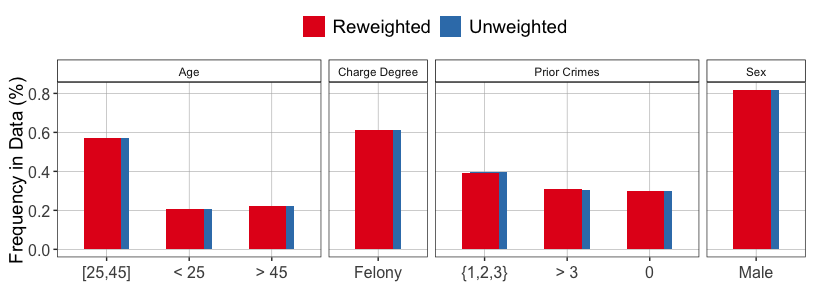
\includegraphics[scale=0.4]{Compas_DP_marginals.png}
\caption{Unweighted vs Reweighted COMPAS dataset. Although the marginals of the two distributions are almost the same, standard fair classifiers show demographic parity of at least $0.1$ on the reweighted dataset.\label{fig:compas-dp-dif}}
\end{figure}

Nonetheless, since different algorithms adopt different definitions of fairness and provide different trade-offs with respect to accuracy and utility, it is neither legal nor ethical to enforce businesses to use such algorithms. In this paper, we approach this problem with a perspective from the literature of automated verification, and aim to build tools that can verify whether an algorithm satisfies a given fairness criteria irrespective of the particular algorithm or dataset used. We show using these tools that, although current group fairness algorithms may mitigate fairness for a specific distribution of data, slight perturbations to that data's distribution result in violations of the fairness criteria. 

\noindent \textbf{Contributions}

\noindent \textbf{Technical Overview}

\noindent \textbf{Experimental Findings}

\noindent \textbf{Related Work}

\section{Problem and Definitions}

We will write $((x,a),y)$ to denote a training instance where $x \in \Xc$ denotes unprotected attributes, $a \in \Ac$ denotes the protected attributes, and $y \in \set{0,1}$ denotes the outcome label. For a hypothesis $h$, $h(x,a) \in \set{0,1}$ denotes the outcome predicted by it. We assume that the set of hypothesis is given by a class $\Hc$. 
Given a loss function $\ell : \set{0,1} \times \set{0,1} \rightarrow \bbR$, the goal of a standard fair classifier is to find a hypothesis $h^* \in \Hc$ that minimizes the training loss $\sum_{i=1}^n \ell(h(x_i,a_i),y_i)$ and is also fair according to some standard fairness criteria. 

In this paper, our goal is different and we wish to find a hypothesis that is fair and robust. We will be designing classifiers that are robust with respect to distributions that are weighted perturbations of the original training distribution. For this, let
 $\WW$ be the set of all possible weights i.e. $\WW = \set{w \in \bbR^+_n : \sum_i w_i = 1}$. For a hypothesis $h$ and weight $w$, we define the following loss function $\ell(h,w) = \sum_{i=1}^n w_i \ell(h(x_i,a_i), y_i)$. We will write  $\delta_F^w(f)$ to define the ``unfairness gap'' with respect to the weighted empirical distribution defined by the weight $w$ and fairness constraint $F$ e.g. demographic parity(DP), equalized odds (EO). For example, $\delta^w_{DP}(f)$ is defined as
\begin{equation}\label{eq:delta-w-dp}
\delta^w_{DP}(f) = \abs{ \frac{\sum_{i: a_i = a} w_i f(x_i,a)}{\sum_{i: a_i = a} w_i} -  \frac{\sum_{i: a_i = a'} w_i f(x_i,a')}{{\sum_{i: a_i = a'} w_i}} }.
\end{equation}
Therefore, $\delta^w_{DP}(f)$ measures the weighted difference in accuracy between the two groups with respect to the training distribution that assigns weight $w$ to the training examples.
On the other hand, $\delta^w_{EO}(f) = \max_{y \in \set{0,1}} \delta^w_{EO}(f|y)$, where $\delta^w_{EO}(f|y)$ is defined as
$$\delta^w_{EO}(f|y) = \abs{ \frac{\sum_{i: a_i = a,y_i = y} w_i f(x_i,a)}{\sum_{i: a_i = a,y_i = y} w_i} -  \frac{\sum_{i: a_i = a',y_i=y} w_i f(x_i,a')}{{\sum_{i: a_i = a',y_i=y} w_i}} }.$$
Therefore, $\delta^w_{EO}(f|0)$ (resp. $\delta^w_{EO}(f|1)$) measures the weighted difference in false (resp. true) positive rates between the two groups with respect to the weight $w$.
%
We will be mainly working with the notion of weighted demographic parity for developing the theory behind our fair and robust classifiers. However, we will provide experimental results concerning both weighted demographic parity, and equalized odds.

We are now ready to formally define our main objective. 
For a class of hypothesis $\HH$, let $\HH_{\WW} = \set{h \in \HH: \delta^w_F(h) \le \epsilon\ \forall w \in \WW}$ be the set of hypothesis that are $\epsilon$-fair with respect to all the weights in the set $\WW$.
Our goal is to solve the following minmax problem:
\begin{equation}\label{eq:det-wt-classification}
\min_{h \in {\HH}_{\WW} } \max_{w \in \WW} \ell(h,w) 
%&\text{s.t. } \delta^w_F(h) \le \epsilon \nonumber
\end{equation}
Therefore, we aim to minimize a robust loss with respect to a class of distributions that are perturbations of the training distribution. Additionally, we also aim to find a classifier that is fair with respect to such perturbations. For our experiments, we will also consider a simplified version of the problem:
\begin{equation}\label{eq:wt-fair-orig}
\min_{h \in {\HH}_{\WW} }  \ell(h,\vec{u}) 
%&\text{s.t. } \delta^w_F(h) \le \epsilon \nonumber
\end{equation}
where $\vec{u}$ is a distribution that assigns uniform weights to all the training points. Contrary to equation \ref{eq:det-wt-classification}, the goal here is to just find a classifier that works well with the original training distribution but is fair with respect to all the weighted perturbations.

We will allow our algorithm to output a classifier which is randomized i.e. it is a distribution over the hypothesis $\HH$. This will also be necessary if the space $\HH$ is non-convex or if the fairness constraints are such that the set of feasible hypothesis $\HH_{\WW}$ is non-convex. For a randomized classifier $\mu$ define the expected loss of $\mu$ as $\ell(\mu,w) = \sum_{h} \mu(h) \ell(h,w)$. 

\section{Design}
We design a robust and fair classifier in a top-down fashion. First we design a meta algorithm that reduces the minmax problem described in equation \ref{eq:det-wt-classification} to a loss minimization problem with respect to a sequence of weight vectors. Then we show how we can design a fair classifier that performs well with respect a fixed weight vector $\vec{w}$ in terms of accuracy, but is fair with respect to the entire class of weights $\WW$.

\subsection{Meta Algorithm}
We now  provide a meta-algorithm that helps us design  fair classifiers that are robust with respect to
any distribution that are some weighted perturbations of the empirical distribution of the training data. The meta-algorithm repeatedly calls an oracle that solves the fair classification problem with respect to a given weighted empirical distribution. 
%In the next section, we will see how to design such an oracle by modifying standard fair classifiers.

\begin{algorithm}[H]
\DontPrintSemicolon
\KwInput{Training Set: $\{x_i,a_i,y_i\}_{i=1}^n$, set of weights: $\WW$, hypothesis class $\HH$, parameters $T$ and $\eta$.}

$w_0(i) = 1/n$ for all $i \in [n]$\\
$h_0 = \AF(w_0)$ \tcc{Approximate solution of $\argmin_{h \in \HH_{\WW}} \sum_{i=1}^n \ell(h(x_i,a_i), y_i)$.}
%$\qquad \text{s.t. } \delta^{w_0}_F(h) \le \epsilon$\\
\For{each $t \in [T]$}
{
	$w_t = w_{t-1} + \eta \nabla_w \ell(h_{t-1},w_{t-1})$\\
	$w_t = \Pi_{\WW}(w_t)$ \tcc{Project $w_t$ onto the set of weights $\WW$.}
	$h_t = \AF(w_t)$ \tcc{Approximate solution of  $\min_{h \in \HH_{\WW}} \sum_{i=1}^n w_t(i) \ell(h(x_i,a_i),y_i)]$.}
	%$\qquad \text{s.t. } \delta^{w_t}_F(h) \le \epsilon$
}
\KwOutput{$h_f$: Uniform distribution over $\set{h_0, h_1,\ldots,h_T}$.}
\caption{Meta-Algorithm\label{algo:meta}}
\end{algorithm}

Algorithm \ref{algo:meta} provides a meta algorithm to solve the min-max optimization problem defined in equation \ref{eq:det-wt-classification}. The algorithm is based on ideas presented in \cite{CLSS17}, which, given an $\alpha$-approximate
Bayesian oracle for distributions over loss functions, provides an $\alpha$-approximate robust solution. %So we assume an access to the following approximate Bayesian oracle.
The algorithm can be viewed as a two-player zero-sum game between the learner who picks the hypothesis $h_t$, and an adversary who picks the weight vector $w_t$. The adversary performs a projected gradient descent every step to compute the best response. On the other hand, the learner solves a fair classification problem to pick the best hypothesis which is fair with respect to the class of weights $\WW$ and minimizes training loss with respect to the weight vector $w_t$. However, it is infeasible to compute an exact optima of the problem $\min_{h \in \HH_{\WW}} \sum_{i=1}^n w_t(i) \ell(h(x_i,a_i),y_i)]$. So the learner uses an approximate fair classifier $\AF(\cdot)$, which we define next.
\begin{definition}\label{def:apx-fair}
$\AF(\cdot)$ is an $\alpha$-approximate fair classifier, if for any weight $w\in\bbR^n_+$, $\AF(w)$ returns a hypothesis $\hat{h}$ such that
$$\sum_{i=1}^n w_i \ell(\hat{h}(x_i,a_i),y_i) \le \min_{h \in \HH_{\WW}} \sum_{i=1}^n w_i \ell(h(x_i,a_i),y_i) + \alpha.$$
\end{definition}

Using the approximate Bayesian oracle, we have the following gurantee on the output of algorithm \ref{algo:meta}. 
\begin{theorem}\label{thm:meta-algo-result}
Suppose the loss function $\ell(\cdot,\cdot)$ is convex in its first argument and $\AF(\cdot)$ is an $\alpha$-approximate fair classifier. Then the ensemble hypothesis $h_f$ output by the meta-algorithm \ref{algo:meta}, satisfies the following:
$$\max_{w \in \WW} \E_{h \sim h_f}\left[ \sum_{i=1}^n w_i \ell(h(x_i,a_i),y_i)\right] \le \min_{h \in {\HH}_{\WW} } \max_{w \in \WW} \ell(h,w) + \max_{w \in \WW} \norm{w}_2 \sqrt{\frac{2}{T}} + \alpha$$
\end{theorem}
The proof of this theorem uses ideas from \cite{CLSS17}, except that we use an additive approximate oracle. 
%\begin{proof}
%Use theorem 7 from \cite{CLSS17}.
%end{proof}

\subsection{Approximate Fair Classifier}
In this section, we develop an $\alpha$-approximate fair and robust classifier. We follow the following three steps to develop such an algorithm, and we belive that this approach might be helpful for developing other robust classifiers.
\begin{enumerate}
\item \label{item:step-a} Discretize the set of all possible weights $\WW$, so that it is sufficient to develop an apporoximate fair classifier with respect to the set of discretized weights. In particular, if we discretize each weight upto an error $\epsilon$, then developoing an $\alpha$-approximate fair classifier with respect to the discretized weights gives $O(\alpha + \epsilon)$-fair classifier wrt the set $\WW$.
\item \label{item:step-b} Set up the problem of designing an approximate fair classifier wrt the set of discretized weights as a two-player zero-sum game. Here, the learner player chooses a hypothesis, whereas an adversary picks the most ``unfair'' weight in the set of discretized weights.
\item \label{item:step-c} Design a learning algorithm for the learner's learning algorithm, and design an approximate solution to adversary's best response to the learner's chosen hypothesis.
\end{enumerate}
We would like to point out that \cite{ABDL+18} was the first to show that the design of a fair classifier can be formulated as a two-player zero-sum game (step \ref{item:step-b}). However, they only considered  group-fairness constraints with respect to the training distribution. On ther other hand, we consider the design of robust and fair classifier and had to include an additional discretization step (\ref{item:step-a}). Finally, the design of our learning algorithm and the best response oracle is significantly different than \cite{ABDL+18,KNRZ17}. For the remainder of this subsection, assume that the meta algorithm (\ref{algo:meta}) called the $\AF(\cdot)$ with a weight vector $w^0$ and our goal is to design a classifier that minimizes weighted loss with respect to the weight $w^0$, but is fair wrt the set of all weights $\WW$ i.e. find $f \in \argmin_{h \in \HH_{\WW} }\ell(h,w^0)$.

\subsubsection{Discretization of the Weights}
We first discretize the set of weights $\WW$. Divide the interval $[0,1]$ into buckets $B_0 = [0,\delta)$, $B_{j+1} = [(1+\gamma_1)^j \delta, (1+\gamma_1)^{j+1}\delta)$ for $j=0,1,\ldots,M-1$ for $M = \ceil{\log_{1+\gamma_1}(1/\delta) )}$. For any weight $w\in \WW$, we construct a new weight $w' = (w'_1,\ldots,w'_n)$ as follows. For each $i \in [n]$, $w'_i$ is the upper-end point of the bucket containing $w_i$. Note that this guarantees that either $w_i\le \delta$ or $\frac{w'_i}{1+\gamma_1} \le w_i \le w_i'$. We now substitute $\delta = \frac{\gamma_1}{2n}$ and write $\Nc(\gamma_1,\WW)$ to denote the set containing all the discretized weights of the set $\WW$.  Now we show that designing fair classifier wrt to the set of weights $\Nc(\gamma_1,\WW)$ is sufficient to designing fair classifier wrt to the set of weights $\WW$. 
\begin{lemma}\label{lem:discrete-weights}
If $\delta^w_{DP}(f) \le \epsilon$ for any weight $w \in \Nc(\gamma_1,\WW)$, then we have $\delta^w_{DP}(f) \le \epsilon + 4\gamma_1$ for any weight $w \in \WW$.
\end{lemma}
 Therefore, in order to ensure that $\delta^w_{DP}(f) \le \eps$ we discretize the set of weights $\WW$ and enforce $\eps-4\gamma_1$ fairness for all the weights in the set $\Nc(\gamma_1,\WW)$. This result makes our work easier as we need to guarantee fairness with respect to a finite set of weights $\Nc(\gamma_1,\WW)$, instead of a large and continuous set of weights $\WW$. However, note that, the number of weights in $\Nc(\gamma_1,\WW)$ can be $O\left( \log^n_{1+\gamma_1}(2n/\gamma_1)\right)$, which can be exponentially large in $n$. We next see how to circumvent this problem.

 \subsection{Setting up a Two-Player Zero-Sum Game}
 %Let us write $N(\gamma_1,\WW)$ to denote the set of all possible such weights vectors. 
 In this section, we set up the problem of designing a fair and robust classifier with respect to the set of weights in $\Nc(\gamma_1,\WW)$ as a two-player zero-sum game. 
 Let us introduce the notation $T(w,a,f) = \frac{\sum_{i: a_i = a} w_i f(x_i,a)}{\sum_{i: a_i = a} w_i}$. Then $\delta^w_{DP}(f) = \sup_{a,a'}\abs{T(w,a,f) - T(w,a',f)}$. 
Now our aim is to solve the following problem.
\begin{align}
&\min_{h \in \HH} \sum_{i=1}^n w^0_i \ell(h(x_i,a_i),y_i)\label{eq:final-objective}\\
&\text{s.t.} T(w,a,h) - T(w,a',h) \le \eps - 4\gamma_1\ \forall w \in N(\gamma_1,\WW) \ \forall a,a' \in \Ac \nonumber
\end{align}
We form the following Lagrangian.
\begin{align}\label{eq:lagrangian}
\min_{h \in \HH} \max_{\lambda : \norm{\lambda}_1 \le B } \sum_{i=1}^n w^0_i \ell(h(x_i,a_i),y_i) + \sum_{w \in N(\gamma_1,\WW)} \sum_{a,a' \in \Ac} \lambda_w^{a,a'} ( T(w,a,h) - T(w,a',h) - \eps + 4\gamma_1)
\end{align}
Notice that we restrict the lagrangian multipliers so that its $L_1$-norm is bounded by the parameter $B$. We will later see how to choose this parameter $B$. In order to solve the minmax problem defined in equation \ref{eq:lagrangian}, we first convert equation \ref{eq:lagrangian} as a two-player zero-sum game. Here the learner's pure strategy is to play a hypothesis $h$ in $\HH$. Given the learner's hypothesis $h\in \HH$, the adversary can pick the constraint that violates fairness the most and set the corresponding coordinate of $\lambda$ to $B$. Therefore, for a fixed hypothesis $h$, it is sufficient for the adversary to play a vector $\lambda$ such that either all the coordinates of $\lambda$ are zero or exactly one is set to $B$. We denote these set of ``pure'' strategies by $\Lambda_p$. Then for any pair of actions $(h,\lambda) \in \HH \times \Lambda_p$, the payoff of the $h$-player of the two-player zero-sum game is defined as
\[U(h,\lambda) = \sum_{i=1}^n w^0_i \ell(h(x_i,a_i),y_i) + \sum_{w \in N(\gamma_1,\WW)} \sum_{a,a' \in \Ac} \lambda_w^{a,a'} ( T(w,a,h) - T(w,a',h) - \eps + 4\gamma_1) \]
Now our goal is to compute a $\nu$-approximate minmax equilibrium of this game. In the next subsection, we will design an algorithm for this problem based on online learning. But we first see how both the $h$-player and the $\lambda$-player compute their best responses. These will be the main components of the learning algorithm discussed later.

\noindent{\bfseries Best response of the $h$-player}: For each $i \in [n]$, we introduce the following notation
$$\Delta_i = \sum_{w \in N(\gamma_1,\WW)} \sum_{a' \neq a_i} \left(\lambda^{a_i,a'}_w - \lambda^{a',a_i}_w \right) \frac{w_i}{\sum_{j:a_j = a_i}w_j}$$
With this notation, the payoff becomes
$$U(h,\lambda) = \sum_{i=1}^n w^0_i \ell(h(x_i,a_i),y_i) + \Delta_i h(x_i,a_i) - (\eps - 4\gamma_1)\sum_{w \in N(\eps/5,\WW)} \sum_{a,a' \in \Ac} \lambda_w^{a,a'}$$
Let us introduce the following costs.
\begin{equation}
c^0_i = \left\{ \begin{array}{cc}
\ell(0,1)w^0_i & \text{ if } y_i = 1\\
\ell(0,0)w^0_i & \text{ if } y_i = 0
\end{array}\right. \quad 
c^1_i = \left\{ \begin{array}{cc}
\ell(1,1)w^0_i + \Delta_i & \text{ if } y_i = 1\\
\ell(1,0)w^0_i + \Delta_i & \text{ if } y_i = 0
\end{array}\right.
\end{equation}
Then the $h$-player's best response becomes the following cost-sensitive classification problem.
\begin{equation}
\hat{h} \in \argmin_{h \in \HH} \sum_{i=1}^n \left\{c^1_i h(x_i,a_i) + c^0_i (1 - h(x_i,a_i)) \right\}
\end{equation}
Therefore, as long as we have access to an oracle that solves the cost-sensitive classification problem, the $h$-player can solve it's best response problem. Note that, the ntion of a cost-sensitive classification as an oracle was also used by \cite{ABDL+18,KNRZ17}. In general, solving this problem is NP-hard, but several efficient implementations are available. We provide further details about how we implement this oracle in the scetion devoted to the experiments.

% \subsection{Equalized Odds}

% We aim is to solve the following problem.
% \begin{align}
% &\min_{h \in \HH} \sum_{i=1}^n w^0_i \ell(h(x_i,a_i),y_i)\label{eq:final-objective}\\
% &\text{s.t.} T(w,a,h,y) - T(w,a',h,y) \le \eps - 4\gamma_1\ \forall w \in N(\gamma_1,\WW) \ \forall a,a' \in \Ac \ \forall y \in \set{0,1} \nonumber
% \end{align}
% Here $T(w,a,h,y) = \frac{\sum_{i:a_i=a,y_i=y} w_i f(x_i,a)}{\sum_{i:a_i=a,y_i=y} w_i}$.
% We form the following Lagrangian.
% \begin{align}\label{eq:lagrangian-eo}
% \min_{h \in \HH} \max_{\stackrel{\lambda }{ \norm{\lambda}_1 \le B} } \sum_{i=1}^n w^0_i \ell(h(x_i,a_i),y_i) + \sum_{w \in N(\gamma_1,\WW)} \sum_{a,a' \in \Ac} \sum_{y} \lambda_w^{a,a',y} ( T(w,a,h,y) - T(w,a',h,y) - \eps + 4\gamma_1)
% \end{align}

% As before, we convert equation \ref{eq:lagrangian-eo} into a two-player zero-sum game. Here the learner's pure strategy is to play a hypothesis $h$ in $\HH$. And the auditor's pure strategy is to play a vector $\lambda$ such that either all the coordinates of $\lambda$ are zero or exactly one is set to $B$. For any pair of actions $(h,\lambda)$, the payoff is defined as
% \[U(h,\lambda) = \sum_{i=1}^n w^0_i \ell(h(x_i,a_i),y_i) + \sum_{w \in N(\gamma_1,\WW)} \sum_{a,a' \in \Ac} \sum_y \lambda_w^{a,a',y} ( T(w,a,h,y) - T(w,a',h,y) - \eps + 4\gamma_1) \]

% For each $i \in [n]$, we introduce the following notation
% $$\Delta_i = \sum_{w \in N(\gamma_1,\WW)} \sum_{a' \neq a_i} \left(\lambda^{a_i,a',y_i}_w - \lambda^{a',a_i,y_i}_w \right) \frac{w_i}{\sum_{j:a_j = a_i, y_j = y_i}w_j}$$
% With this notation, the payoff becomes
% $$U(h,\lambda) = \sum_{i=1}^n w^0_i \ell(h(x_i,a_i),y_i) + \Delta_i h(x_i,a_i) - (\eps - 4\gamma_1)\sum_{w \in N(\eps/5,\WW)} \sum_{a,a' \in \Ac} \sum_y \lambda_w^{a,a',y}$$

\noindent{\bfseries Best response of the $\lambda$-player}: Given a hypothesis $h\in \HH$, the best response of the $\lambda$-player is simple -- find the weight in $\Nc(\gamma_1,\WW)$ that violates the fairness constraint most and set that coordinate to $B$. However, finding such a constraint is a non-linear optimization problem because the fairness constraints depend on the weights non-linearly (e.g. see definition of demographic parity in eq. \ref{eq:delta-w-dp}). However, we show that an approximate best response can be computed by solving a system of
linear programs. The idea is that we can guess the marginal probabilities over the protected groups. If we are correct, then the most violating weight vector for demographic parity can be found by a linear program. Since we cannot exactly guess this particular value, we instead discretize the set of marignal probabilities, iterate over them and choose the option with largest violation in fairness.

The above intuition can be formalized as follows.
%
We first discretize the set of all marginals over the groups i.e. the simplex over $\abs{\Ac}$.
%, $\Delta_{\Ac} = \set{\pi \in \bbR^{\abs{\Ac}}_+: \sum_{a \in \Ac} \pi_a = 1}$. 
For example, we discretize $[0,1]$ as $0,\delta, (1+\gamma_2)^j \delta$ for $j=1,2,\ldots,M$ for $M = O(\log_{1+\gamma_2}(1/\delta))$. This discretizes $[0,1]^{\Ac}$ into $M^{\abs{\Ac} }$ points, and then we retain the discretized marginals whose total sum is at most $1+\gamma_2$, and discard all other points. Let us denote the set of such marginals as $\Pi(\gamma_2,\Ac)$. Algorithm \ref{algo:best-lambda} describes the best response of the $\lambda$-player for a given choice of hypothesis $h$. It goes through all the marginals $\pi$ in $\Pi(\gamma_2,\Ac)$ and for each such tuple and a pair of groups $a,a'$ finds the weight $w$ which maximizes $T(w,a,h) - T(w,a',h)$. Note that this can be solved using a Linear Program as the weights assigned to a group is fixed by the marginal tuple $\pi$. Out of all the solutions, the algorithm finds the one with the maximum value. Then it checks whether this maximum violates the constraint i.e. greater than $\eps - 4\gamma_1$. If so, it sets the corresponding $\lambda$ value to $B$ and everything else to $0$. Otherwise, it returns the zero vector. Note that, the weight returned by the linear program need not correspond to a weight in $\Nc(\gamma_1, \WW)$. In that case, the algorithm rounds the weight to the nearest weight in $\Nc(\gamma_1,\WW)$ and sets the corresponding $\lambda$ variable to $B$. For discretizing the marginals we will set $\delta = (1+\gamma_2)\frac{\gamma_1}{n}$, which implies that the number of LP-s run by algorithm \ref{algo:best-lambda} is at most $O\left(\log^{\abs{\Ac}}_{1+\gamma_2}\left( \frac{n}{(1+\gamma_2)\gamma_1}\right)\right) = O(\textrm{poly}(\log n))$, as the number of groups is fixed.

\begin{algorithm}[H]
\DontPrintSemicolon
\KwInput{Training Set: $\{x_i,a_i,y_i\}_{i=1}^n$, and hypothesis $h \in \HH$.}
%\KwInput{Training Set: $\{x_i,a_i,y_i\}_{i=1}^n$, set of weights: $\WW$, hypothesis class $\HH$, parameters $T$ and $\eta$.}
\For{each $\pi \in \Pi(\gamma_2,\Ac)$}
{
	\For{each $a,a' \in \Ac$}
	{
	Solve the following LP:
	\begin{align*}
	w(a,a',\pi) = \argmax_w \quad &\frac{1}{\pi_a} \sum_{i:a_i = a} w_i h(x_i,a) - \frac{1}{\pi_{a'}} \sum_{i:a_i = a'} w_i h(x_i,a') \\
	\textrm{s.t.} \quad & \sum_{i:a_i = a} w_i  = \pi_a \quad 
 \sum_{i: a_i = a'} w_i = \pi_{a'} \quad
 w_i \ge 0 \quad \forall i \in [n] \quad
\sum_{i=1}^n w_i = 1
	\end{align*}
	Set $\textrm{val}(a,a',\pi) = \frac{1}{\pi_a} \sum_{i:a_i = a} w(a,a',\pi)_i h(x_i,a) - \frac{1}{\pi_{a'}} \sum_{i:a_i = a'} w(a,a',\pi)_i h(x_i,a')$\\
	}
}
Set $(a^*_1,a^{*}_2,\pi^*) = \argmax_{a,a',\pi} \text{val}(a,a',\pi)$\\
\uIf{$\textrm{val}(a^*_1,a^{*}_2,\pi^*) > \eps$}
{
	Let $w = w(a^*_1,a^{*}_2,\pi^*)$.\\
	For each $i \in [n]$, let $w_i'$ be the upper-end point of the bucket containing $w_i$.\\
	\Return{$\lambda^{a,a'}_w = \left\{ \begin{array}{cc}
	B & \text{ if } (a,a',w) = (a^*_1,a^{*}_2,w') \\
	0 & \text{ o.w. }
	\end{array}\right.$}
}
\uElse{
	\Return{$\vec{0}$}
}
\caption{Best Response of the $\lambda$-player\label{algo:best-lambda}}
\end{algorithm}

The next lemma shows that algorithm \ref{algo:best-lambda} computes an approximate best-response for the $\lambda$-player.
\begin{lemma}
Algorithm \ref{algo:best-lambda} is an $B(4\gamma_1 + \gamma_2)$-approximate best response for the $\lambda$-player i.e. for any $h \in \HH$, it returns $\lambda^*$ such that
$U(h,\lambda^*) \ge \max_{\lambda} U(h,\lambda) - B(4\gamma_1 + \gamma_2)$.
\end{lemma}

\noindent{\bfseries Learning Algorithm}:
 We are now ready to introduce our algorithm for the problem defined in equation \ref{eq:lagrangian}. In this algorithm, the $h$-player will use a learning algorithm, but the $\lambda$-player will use algorithm \ref{algo:best-lambda} to compute its approximate best response. The learning algorithm will use the Regularized Follow the Leader (RFTL) algorithm and we now briefly review this algorithm and its guarantees. RFTL is a classical algorithm for online convex optimization (OCO). In OCO, the decision maker takes a decision $x_t \in \Kc$ at round $t$, an adversary reveals a convex loss function $f_t:\Kc \rightarrow \bbR$, and the decision maker suffers a loss of $f_t(x_t)$. The goal is to minimize regret, which is defined as $\max_{u \in \Kc}\left\{\sum_{t=1}^T f_t(x_t) - f_t(u)\right\}$ i.e. the difference between the loss suffered by the learner and the best fixed decision that could have been made in hindsight. RFTL algorithm requires a strongly convex regularization function $R:\Kc \rightarrow \bbR_{\ge 0}$ chooses $x_t$ according to the following rule:
$$x_{t} = \argmin_{x \in \Kc} \left\{\eta \sum_{s=1}^{t-1} \nabla f_s(x_s)^T x + R(x)  \right\}.$$
The interested reader is referred to the textbook by \cite{Hazan16} for details about RFTL and guarantees on its performance.

% \begin{algorithm}[H]
% \DontPrintSemicolon
% \KwInput{$\eta > 0$, regularization function $R$, and a convex compact set $\Kc$.}
% Set $x_1 = \argmin_{x \in \Kc}R(x)$\\
% %$\qquad \text{s.t. } \delta^{w_0}_F(h) \le \epsilon$\\
% \For{$t \in [T]$}
% {
% 	Predict $x_t$\\
% 	Observe $f_t$ and compute $\nabla f_t(x_t)$\\
% 	Update $$x_{t+1} = \argmin_{x \in \Kc} \left\{\eta \sum_{s=1}^t \nabla f_t(x_t)^T x + R(x)  \right\}$$\\
% 	%$\qquad \text{s.t. } \delta^{w_t}_F(h) \le \epsilon$
% }
% \caption{RFTL}
% \end{algorithm}

% \begin{theorem}\label{thm:rftl-guarantee}
% The RFTL algorithm achieves the following regret bound for any $u \in \Kc$
% $$\sum_{t=1}^T f_t(x_t) - f_t(u) \le \frac{\eta}{4} \sum_{t=1}^T \norm{\nabla f_t(x_t)}_{\infty}^{2} + \frac{R(u) - R(x_1)}{2 \eta}$$
% Moreover, if $\norm{\nabla f_t(x_t)}_{\infty} \le G_R$ for all $t$ and $R(u) - R(x_1) \le D_R$ for all $u \in \Kc$, then we can optimize $\eta$ to get the following bound: $\sum_{t=1}^T f_t(x_t) - f_t(u) \le D_R G_R \sqrt{T}$.
% \end{theorem}

We now use RFTL algorithm to design an algorithm (\ref{algo:inner}) for solving a minmax approximate equilibrium of the game $U(h,\lambda)$. 
The $h$-player uses RFTL as a learning algorithm to choose $h_t$, whereas the $\lambda$-player uses algorithm \ref{algo:best-lambda} to generate an approximate best response $\lambda_t$ to $h_t$. Recall that, in order to use the RFTL algorithm we need to specify the regularization function $R$ and cost function $f_t$ in each round. We choose $R(x) = 1/2\norm{x}_2^2$. At round $t$, for an action $h_t$, the cost function is $f_t(h_t) = U(h_t,\lambda_t)$ where $\lambda_t$ is the approximate best-response to $h_t$. Therefore, in order to implement RFTL the learner needs to solve the following optimization problem. 
\begin{equation}\label{eq:optim-step}
h_t \in \argmin_{h \in \HH}\left\{\eta \sum_{s=1}^{t-1}\nabla_{h_s} U(h_s,\lambda_s)^T h + \frac{1}{2}\norm{h}_2^2\right\}
\end{equation}
Here with slight abuse of notation we write $\HH$ to include the set of randomized classifiers. So that $h(x_i,a_i)$ is interpreted as the probability that hypothesis $h$ outputs $1$ on an input $(x_i,a_i)$. Now we show that the optimization problem (eq. \ref{eq:optim-step}) faced by the learner becomes a cost-sensitive classification problem. Recall that given $\lambda_s$, the best response of the learner is given by the following cost-sensitive classification problem.
\begin{equation*}
\hat{h} \in \argmin_{h \in \HH} \sum_{i=1}^n c^1_i (\lambda_s) h(x_i,a_i) + c^0_i(\lambda_s) (1 - h(x_i,a_i))
\end{equation*}
We now use a linearization trick used by \cite{KNRZ17}.
Writing $L_i(\lambda_s) = c^1_i(\lambda_s) - c^0_i(\lambda_s)$, the objective in the problem above becomes $\sum_{i=1}^n L_i(\lambda_s) h(x_i,a_i)$. Hence, $\nabla_{h_s}U(h_s,\lambda_s)$ is linear in $h_s$ and equals the vector $\{L_i(\lambda_s)\}_{i=1}^n$. With this observation, the objective in equation \ref{eq:optim-step} becomes
%{\bfseries Best Respose to $\lambda$}: For a given set of lagrangian multipliers $\{\lambda_w\}_{w \in N(\eps/5,\WW)}$, the optimal choice of $h$ is a weighted classification problem. 
% Algorithm \ref{algo:inner} describes the algorithm for solving a minmax approximate equilibrium of the game $U(h,\lambda)$ for $h \in \HH$ and $\lambda \in \bbR^{\abs{N(\gamma_1,\WW)}\times \abs{\Ac}^2}_+, \norm{\lambda}_1 \le B$. We will later see how this solution immediately leads to a solution for the optimization problem defined in equation \ref{eq:final-objective}. The $h$-player uses the RFTL algorithm as a learning algorithm whereas the $\lambda$-player approximately best respond to $h_t$ in each round. Recall that, in order to use the RFTL algorithm we need to specify the regularization function $R$ and cost function $f_t$ in each round. We choose $R(x) = 1/2\norm{x}_2^2$. As the learner always chooses a vector in $\set{0,1}^n$ corresponding to the $n$ predictions for the $n$ training instances, the diameter $D_R$ is bounded by $n$. At round $t$, for an action $h_t$, the cost function is $f_t(h_t) = U(h_t,\lambda_t)$ where $\lambda_t$ is the $B(4\gamma_1 + \gamma_2)$-approximate best-response to $h_t$. Now we show that the optimization problem faced by the learner becomes a cost-sensitive classification problem. Indeed,
\begin{align*}
&= \eta \sum_{s=1}^t \sum_{i=1}^n L(\lambda_s) h(x_i,a_i) + \frac{1}{2} \sum_{i=1}^n (h(x_i,a_i))^2 \\
&\le \eta \sum_{i=1}^n L\left(\sum_{s=1}^t \lambda_s\right) h(x_i,a_i) + \frac{1}{2} \sum_{i=1}^n h(x_i,a_i) \\
&= \sum_{i=1}^n \left(\eta L\left(\sum_{s=1}^t \lambda_s\right) + \frac{1}{2}\right) h(x_i,a_i)
\end{align*}
The second inequality follows from two observations. First, $L(\lambda)$ is linear in $\lambda$. Second, since the predictions $h(x_i,a_i) \in [0,1]$ we replace the quadratic term by a linear term, an upper bound\footnote{Without this relaxation we will be solving a regularized version of cost-sensitive classification}. We would like to contrast our approach with \cite{KNRZ17}, who used Follow the Perturbed Leader (FTPL) algorithm for the learner. Our approach has several benefits.
\begin{enumerate}
\item Since RFTL doesn't use randomized regularization, the predictions generated by our method are more robust. \dm{Rephrase.}
\item We will use RFTL based learning algorithm to design a fast solver for the minmax objective.
\end{enumerate}
Finally, we observe that even though the number of $\lambda$-variables is exponential in $n$, the algorithm can be efficiently implemented. In fact, the best response of the $\lambda$-player always returns a solution where all the variables are zero or exactly one is set to $B$. Therefore, instead of recording the entire $\lambda$ vector the learning algorithm can just record the non-zero variables and there will be at most $T$ of them. The next lemma provides performance guarantees of algorithm \ref{algo:inner}.
\begin{algorithm}
\DontPrintSemicolon
\KwInput{$\eta > 0$, weight $w^0 \in \bbR^n_+$, number of rounds $T$}
Set $h_1 = 0$\\
\For{$t \in [T]$}
{
	$\lambda_t = \text{Best}_{\lambda}(h_t)$\\
	Set $\tilde{\lambda}_t = \sum_{t'=1}^t \lambda_{t'}$\\
	$h_{t+1} = \argmin_{h \in \HH} \sum_{i=1}^n (\eta L_i(\tilde{\lambda}_t) + 1/2) h(x_i,a_i)$ %\tcc{Upper Bound of }
}
\Return{Uniform distribution over $\set{h_1,\ldots,h_T}$.}
\caption{Approximate Fair Classifier ($\AF$)\label{algo:inner}}
\end{algorithm}
\begin{theorem}
Given a desired fairness level $\eps$, if algorithm \ref{algo:inner} is run for $T= O\left(\frac{n}{\eps^2} \right)$ rounds, then the ensemble hypothesis $\hat{h}$ provides the following guarantees:
$$\sum_{i=1}^n w^0_i \ell(\hat{h}(x_i,a_i),y_i) \le \min_{h \in \HH}\sum_{i=1}^n w^0_i \ell({h}(x_i,a_i),y_i) + O(\eps)
\ \textrm{and} \ 
 \delta^w_{DP}(\hat{h}) \le 2\eps \quad \forall w \in \WW.$$
\end{theorem}

\section{Faster Approximate Fair Classifier}

\section{Experiment}

\section{Conclusion}

\bibliographystyle{plainnat}
\bibliography{newrefs}

\appendix
\section{Appendix}

\begin{lemma}
If $\delta^w_{DP}(f) \le \epsilon$ for any weight $w \in \Nc(\gamma_1,\WW)$, then we have $\delta^w_{DP}(f) \le \epsilon + 4\gamma_1$ for any weight $w \in \WW$.
\end{lemma}
\begin{proof}
Recall the definition of demographic parity with respect to a weight vector $w$.
$$\delta^w_{DP}(f) = \abs{ \frac{\sum_{i: a_i = a} w_i f(x_i,a)}{\sum_{i: a_i = a} w_i} -  \frac{\sum_{i: a_i = a'} w_i f(x_i,a')}{{\sum_{i: a_i = a'} w_i}} }$$ 
For a given weight $w$, we construct a new weight $w' = (w'_1,\ldots,w'_n)$ as follows. For each $i \in [n]$, $w'_i$ is the upper-end point of the bucket containing $w_i$. Note that this guarantees that either $w_i\le \delta$ or $\frac{w'_i}{1+\gamma_1} \le w_i \le w_i'$. We now establish the following lower bound.
\begin{align}\label{eq:lbd-ratio}
\frac{\sum_{i: a_i = a} w_i f(x_i,a)}{\sum_{i: a_i = a} w_i} \ge \frac{1}{1+\gamma_1}  \frac{\sum_{i: a_i = a} w_i' f(x_i,a)}{\sum_{i: a_i = a} w_i'} \ge (1-\gamma_1) \frac{\sum_{i: a_i = a} w_i' f(x_i,a)}{\sum_{i: a_i = a} w_i'} 
\end{align}
Also note that,
\begin{align*}
\sum_{i: a_i = a} w_i' &\le \sum_{i:a_i = a, w_i > \delta} w_i + \sum_{i: a_i = a, w_i \le \delta} \delta 
\le (1+\gamma_1) \sum_{i:a_i = a, w_i > \delta} w_i' + n \delta
\end{align*}
This gives us the following.
\begin{align*}
\frac{\sum_{i: a_i = a} w_i f(x_i,a)}{\sum_{i: a_i = a} w_i} \le \frac{\sum_{i: a_i = a} w_i' f(x_i,a)}{\frac{1}{1+\gamma_1}\sum_{i: a_i = a} w_i' - \frac{n\delta}{1+\gamma_1} }  \le (1+\gamma_1) \frac{\sum_{i: a_i = a} w_i' f(x_i,a)}{\sum_{i: a_i = a} w_i' - n\delta } 
\end{align*}
Now we substitute, $\delta=\gamma_1/(2n)$ and get the following upper bound.
\begin{align}%\label{eq:ubd-ratio}
\frac{\sum_{i: a_i = a} w_i f(x_i,a)}{\sum_{i: a_i = a} w_i} &\le (1+\gamma_1) \frac{\sum_{i: a_i = a} w_i' f(x_i,a)}{\sum_{i: a_i = a} w_i' - \gamma_1/2}\nonumber \\ &\le \frac{1+\gamma_1}{1-\gamma_1} \frac{\sum_{i: a_i = a} w_i' f(x_i,a)}{\sum_{i: a_i = a} w_i'} \le (1+3\gamma_1)  \frac{\sum_{i: a_i = a} w_i' f(x_i,a)}{\sum_{i: a_i = a} w_i'}\label{eq:ubd-ratio}
\end{align}
% \begin{align*}
% &\frac{\sum_{i: a_i = a} w_i f(x_i,a) - \norm{w - w'}_1}{\sum_{i: a_i = a} w_i + \norm{w - w'}_1} \le \frac{\sum_{i: a_i = a} w_i f(x_i,a)}{\sum_{i: a_i = a} w_i} \le \frac{\sum_{i: a_i = a} w_i f(x_i,a) + \norm{w - w'}_1}{\sum_{i: a_i = a} w_i - \norm{w - w'}_1} \\
% \iff &\frac{\sum_{i: a_i = a} w_i f(x_i,a) - \eps/4}{\sum_{i: a_i = a} w_i + \eps/4} \le \frac{\sum_{i: a_i = a} w_i f(x_i,a)}{\sum_{i: a_i = a} w_i} \le \frac{\sum_{i: a_i = a} w_i f(x_i,a) + \eps/4}{\sum_{i: a_i = a} w_i - \eps/4} \\
% \iff & \frac{\sum_{i: a_i = a} w_i f(x_i,a) - \eps/4}{1/2\sum_{i: a_i = a} w_i} \le \frac{\sum_{i: a_i = a} w_i f(x_i,a)}{\sum_{i: a_i = a} w_i} \le  \frac{\sum_{i: a_i = a} w_i f(x_i,a) + \eps/4}{1/2\sum_{i: a_i = a} w_i}
% \end{align*}
Now we bound $\delta^w_{DP}(f)$ using the results above. Suppose $\frac{\sum_{i: a_i = a} w_i f(x_i,a)}{\sum_{i: a_i = a} w_i} >  \frac{\sum_{i: a_i = a'} w_i f(x_i,a')}{\sum_{i: a_i = a'} w_i}$. Then we have,
%\begin{align*}
%\delta^w_{DP}(f) = \frac{\sum_{i: a_i = a} w_i f(x_i,a)}{\sum_{i: a_i = a} w_i} -  \frac{\sum_{i: a_i = a'} w_i f(x_i,a')}{\sum_{i: a_i = a'} w_i}
%\end{align*}
%Then we have,
\begin{align*}
\delta^w_{DP}(f) &\le (1+3\gamma_1)  \frac{\sum_{i: a_i = a} w_i' f(x_i,a)}{\sum_{i: a_i = a} w_i'} - (1-\gamma_1) \frac{\sum_{i: a_i = a} w_i' f(x_i,a)}{\sum_{i: a_i = a} w_i'}  \\
&\le  \frac{\sum_{i: a_i = a} w_i' f(x_i,a)}{\sum_{i: a_i = a} w_i'} -  \frac{\sum_{i: a_i = a} w_i' f(x_i,a)}{\sum_{i: a_i = a} w_i'} + 4\gamma_1\\
&\le \delta^{w'}_{DP}(f) + 4\gamma_1
\end{align*}
The first inequality uses the upper bound for the first term (eq. \ref{eq:ubd-ratio}) and the lower bound for the second term (eq. \ref{eq:lbd-ratio}). The proof when the first term is less than the second term in the definition of $\delta^w_{DP}(f)$ is similar. Therefore, if we guarantee that $\delta^{w'}_{DP}(f) \le \eps$, we have $\delta^w_{DP}(f) \le \eps+4\gamma_1$.
\end{proof}

\end{document}
